\documentclass[A4paper, 11pt]{article}
\usepackage[a4paper, total={7.2in, 10.5in}]{geometry}
\usepackage{tikz}
\usetikzlibrary{calc}
\usepackage{setspace}
\usepackage{graphicx}
\usepackage{amsmath}
\usepackage{pgfplots}
\graphicspath{ {./images/} }
\usepackage{bookmark}
\setcounter{tocdepth}{3}
\DeclareMathOperator\cosec{cosec}

\title{A Level Mathematics - Statistics}
\author{Xingzhi Lu}
\date{For exam in 2025}

\usepackage{mathptmx}

\begin{document}
	\maketitle
	\section{Statistical sampling}
	
	\subsection{Populations and samples}
	\subsubsection{Definitions}
	\begin{description}
		\item[Population:] The whole set of items that are of interest
		\item[Census:] Observes or measures every member of a population
		\item[Sample:] A selection of observations taken from a subset of the population which is used
		\item[Sampling unit:] Individual units of a population that cam be sampled
		\item[Sampling frame:] A list of all people or item that can potentially be involved in the sample
	\end{description}
	
	\subsubsection{Census}
	\textbf{Advantages}
	\begin{itemize}
		\item Gives a completely accurate result, no bias
	\end{itemize}
	\textbf{Disadvantages}
	\begin{itemize}
		\item Time consuming and expensive
		\item Cannot be used when the testing process destroys the item
		\item Hard to process large quantity of data
	\end{itemize}
	\subsubsection{Sample}
	\textbf{Advantages}
	\begin{itemize}
		\item Easier to implement
		\item Quicker to implement
		\item Less data to process
	\end{itemize}
	\textbf{Disadvantages}
	\begin{itemize}
		\item The data may not be representative
		\item The sample may not be large enough to give information about small sub-groups of the population
	\end{itemize}
	\subsubsection{Sample size}
	\begin{itemize}
		\item Larger sample size = better accuracy
		\item If the population is varied a larger sample size is needed to make sure that the sample is representative
	\end{itemize}
	
	
	\subsection{Random sampling methods}
	\subsubsection{Simple random sampling}
	\textbf{Definition}
	\begin{itemize}
		\item Every possible sample of size $n$ has an \textbf{equal chance} of being picked
	\end{itemize}
	\textbf{Method}
	\begin{enumerate}
		\item Each sampling unit is numbered from 1 to $n$
		\item Generate $x$ random number between 1 to $n$ using random number generators / lottery picks / random number tables (or draw out $x$ names from the lottery hat)
		\item Sampling units corresponding to these numbers become the sample
		\item Data taken from the sample
	\end{enumerate}
	\textbf{Advantages}
	\begin{itemize}
		\item Free of bias
		\item Easy and cheap to implement for small populations and small samples
		\item Each sampling unit has a known and equal chance of selection
	\end{itemize}
	\textbf{Disadvantages}
	\begin{itemize}
		\item Not suitable when the population size or the sample size is large as it is potentially time consuming, disruptive and expensive
		\item A sampling frame is needed
	\end{itemize}
	\subsubsection{Systematic sampling}
	\textbf{Definition}
	\begin{itemize}
		\item The required elements are chosen at \textbf{regular intervals} from an \textbf{ordered list}
	\end{itemize}
	\textbf{Method}
	\begin{enumerate}
		\item The population is ordered with a unique number each from 1 to $n$
		\item Required elements are chosen at regular intervals i.e. take every $k$th elements where $k=\dfrac{\text{Population size}}{\text{Sample size}}$
		\item Starting at random item between 1 and $k$ using a random number generator
		\item Select the remaining data at the chosen interval
	\end{enumerate}
	\textbf{Advantages}
	\begin{itemize}
		\item Simple and quick to use
		\item Suitable for large samples and large populations
	\end{itemize}
	\textbf{Disadvantages}
	\begin{itemize}
		\item A sampling frame is needed
		\item It can introduce bias if the sampling frame is not random
	\end{itemize}
	\subsubsection{Stratified sampling}
	\textbf{Definition}
	\begin{itemize}
		\item The population is divided into mutually exclusive strata and a random sample is taken from each
	\end{itemize}
	\textbf{Method}
	\begin{enumerate}
		\item Population divided into \textbf{non-overlapping} groups / strata
		\item Same proportion ($\dfrac{\text{Sample size}}{\text{Population size}}$) sampled from each strata (work out the total population and the size of each strata individually, round if needed)
		\item Simple random sampling carried out in each group (explain in more details here)
	\end{enumerate}
	\textbf{Advantages}
	\begin{itemize}
		\item Sample accurately reflects the population structure
		\item Guarantees proportional representation of groups within a population
	\end{itemize}
	\textbf{Disadvantages}
	\begin{itemize}
		\item Population must be clearly classified into distinct strata
		\item Selection within each stratum suffers from the same disadvantages as simple random sampling
	\end{itemize}
	\subsection{Non-random sampling methods}
	\subsubsection{Quota sampling}
	\textbf{Method}
	\begin{enumerate}
		\item Population divided into groups according to a given characteristic
		\item A quota group is set to try and reflect the group's proportion in the whole population
		\item An interviewer or researcher selects a sample that reflects the characteristics of the whole population (opportunity sampling)
	\end{enumerate}
	\textbf{Advantages}
	\begin{itemize}
		\item Allows a small sample to still be representative of the population
		\item No sampling frame required
		\item Quick, easy, inexpensive
		\item Allows for easy comparison between different groups of population
	\end{itemize}
	\textbf{Disadvantages}
	\begin{itemize}
		\item Non-random sampling can introduce bias
		\item Population must be divided into groups, which can be costly or inaccurate
		\item Increasing scope of study increases number of groups, adding time or expense
		\item Non-responses are not recorded
	\end{itemize}
	
		\subsubsection{Opportunity / convenience / pragmatic sampling}
	\textbf{Method}
	\begin{enumerate}
		\item Sample taken from people who are available at time of study and meet the criteria
	\end{enumerate}
	\textbf{Advantages}
	\begin{itemize}
		\item Easy to carry out
		\item No sampling frame required
		\item Inexpensive
	\end{itemize}
	\textbf{Disadvantages}
	\begin{itemize}
		\item Likely to be unrepresentative
		\item Highly dependent on individual researcher
	\end{itemize}
	
	\section{Data presentation and interpretation}
	\subsection{Types of data}
	\begin{description}
		\item[Quantitative data:] Associated with numerical observations
		\item[Qualitative data:] Associated with non-numerical observations
		\item[Continuous data:] Can take any value in a given range
		\item[Discrete data:] Can only take specific values in a given range
	\end{description}
	
	\subsection{Linear regression}
	* Work these out using a calculator in exams
	\subsubsection{Regression equation}
	\begin{itemize}
		\item $\hat{y}=ax+b$
		\item $a=\dfrac{S_{\mathrm{xy}}}{S_{\mathrm{xx}}}=\dfrac{\sum (x_i-\overline{x}) (y_i-\overline{y})}{\sum (x_i-\overline{x})^2}$
		\item $b=\overline{y}-a\overline{x}$
	\end{itemize}
	
	\subsubsection{PMCC}
	\begin{itemize}
		\item Measures the strength of \textbf{linear} correlation
		\item  $r =\dfrac{\sum\left(x_{i}-\bar{x}\right)\left(y_{i}-\bar{y}\right)}{\sqrt{\sum\left(x_{i}-\bar{x}\right)^{2} \sum\left(y_{i}-\bar{y}\right)^{2}}}$
	\end{itemize}
	
	\subsection{Interpreting distributions}
	\begin{description}
		\item[Measuring central tendency:] Mean / median / mode
		\item[Measuring spread of data:] Variance / standard deviation / range / interpercentile ranges
	
	\end{description}
	
	\subsubsection{Standard deviation / variance}
	\begin{itemize}
		\item $S_{xx}=\Sigma (x-\overline{x})^2=\Sigma x^2 - \dfrac{(\Sigma x)^2}{n}$
		\item $Var(x)=E(x^2)-(E(x))^2=E((x- E(x) )^2)$
		\item $\sigma=\sqrt{\dfrac{S_{xx}}{n}}=\sqrt{\dfrac{\Sigma x^2}{n} - (\dfrac{\Sigma x}{n})^2}$
	\end{itemize}
	
	\subsubsection{Sample variance}
	\begin{itemize}
		\item $S^2=\dfrac{\Sigma(x_i-\overline{x})^2}{n-1}=\dfrac{1}{n-1}(\Sigma x_i^2-\overline{x}^2n)=\dfrac{1}{n-1}(\Sigma x_i^2-\dfrac{(\Sigma x)^2}{n})$
	\end{itemize}

	
	\subsection{Transform to linear regression}
	\subsubsection{Exponential}
	\begin{itemize}
		\item $y=ab^x\rightarrow\ln y = x\ln b + \ln a$
		\item x-axis = $x$, y-axis = $\ln y$, gradient = $\ln b$, y-intercept = $\ln a$
	\end{itemize}
	\subsubsection{Power}
	\begin{itemize}
		\item $y=ax^b\rightarrow\ln y = b\ln x + \ln a$
		\item x-axis = $\ln x$, y-axis = $\ln y$, gradient = $b$, y-intercept = $\ln a$
	\end{itemize}
	
	\subsubsection{Logarithmic}
	\begin{itemize}
		\item $y=a\ln x\rightarrow$ kept the same
		\item x-axis = $\ln x$, y-axis = $y$, gradient = $a$
	\end{itemize}
	
	
	\subsection{Large data set}
	\subsubsection{Scope}
	\begin{itemize}
		\item Months included: May - October
		\item Years included: 2015 and 1987
	\end{itemize}
	\subsubsection{Cities}
	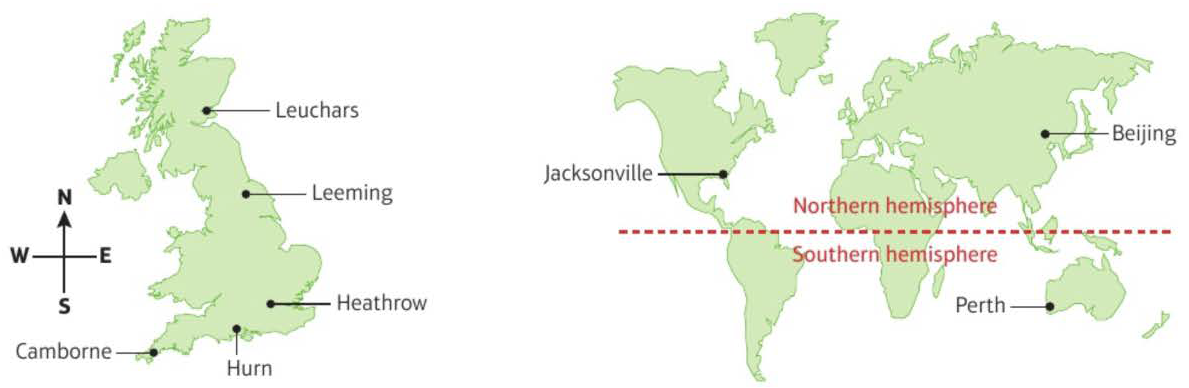
\includegraphics{LDSmap}\\
	Ordered from north to south:
	\begin{enumerate}
		\item Leuchars
		\item Leeming
		\item Heathrow
		\item Hurn
		\item Camborne
		\item Beijing
		\item Jacksonville
		\item Perth (Southern hemisphere)
	\end{enumerate}
	
	\subsubsection{Data recorded}
	\begin{tabular}{|c|c|c|c|c|c|}
		\hline
		\textbf{Variable} & \textbf{Unit} & \textbf{Precision}\\
		\hline
		Daily mean temperature & Celsius & to 1 dp\\
		\hline
		Daily total rainfall & mm & to 1 dp (tr = less than 0.05 mm, treat as 0)\\
		\hline
		Daily total sunshine & hours & to 1 dp \\
		\hline
		Daily maximum relative humidity & as a percentage & nearest integer \\
		\hline
		Daily mean wind direction & degree + cardinal direction & nearest integer  \\
		\hline
		Daily mean windspeed & knots / Beaufort conversion & nearest integer \\
		\hline
		Daily maximum gust & knots & nearest integer   \\
		\hline
		Daily maximum gust direction & degree + cardinal direction & nearest integer   \\
		\hline
		Daily mean cloud cover & oktas  & integer from 0-8   \\
		\hline
		Daily mean visibility & decametres (Dm) & nearest 100  \\
		\hline
		Daily mean pressure & hectopascals (hPa) & nearest integer  \\
		\hline
	\end{tabular}
	


	
	\section{Statistical distributions}
	\subsection{Binomial distribution}
	\subsubsection{Notation}
	$X \sim B(n,p)$
	\subsubsection{Probability calculation}
	$\text{P}(x) = \dbinom{n}{x} p^x q^{n-x}$
	\subsubsection{Assumptions}
	\begin{itemize}
		\item There are a fixed number of trials, $n$
		\item There are two possible outcomes only (success and failure)
		\item There is a fixed probability of success, $p$
		\item The trials are independent of each other
	\end{itemize}
	\subsubsection{Approximation of binomial distribution}
	If $n$ is large ($n\geq35$) and $p$ is close to $0.5$, then $X \sim N(np, np(1-p))$\\
	When estimating probability $(n\in \textbf{N})$:
	\begin{itemize}
		\item $\text{P}(X>n)\approx \text{P}(X>[n+0.5])$
		\item $\text{P}(X\geq n)\approx \text{P}(X\geq [n-0.5])$
		\item $\text{P}(X=n)\approx \text{P}([n-0.5]<X<[n+0.5])$
		\item $\text{P}(X<n)\approx \text{P}(X<[n-0.5])$
		\item $\text{P}(X \leq n)\approx \text{P}(X\leq [n+0.5])$
	\end{itemize}
	
	\subsection{Normal distribution}
	\subsubsection{Notation}
	$X \sim N(\mu,\sigma^2)$
	\subsubsection{Conditions}
	\begin{itemize}
		\item Mean = median = mode
		\item Continuous variable
		\item Symmetrical distribution
	\end{itemize}
	\subsubsection{Shape of distribution}
	\begin{itemize}
		\item Symmetrical shape (mean = median = mode)
		\item Bell-shaped curve with asymptotes at each end
		\item Total area under curve = $1$
		\item Has points of inflection at $\mu+\sigma$ and $\mu-\sigma$
		\item Approximately 68\% of data lies within 1 s.d. from mean, 95\% within 2 s.d., 99.7\% (nearly all) within 3 s.d.
	\end{itemize}
	
	
	\section{Hypothesis testing}
	\subsection{Definitions}
	\begin{description}
		\item[Null hypothesis $H_0$:] $\theta=\theta_0$
		\item[Alternative hypothesis $H_1$:] $\theta \neq \theta_0$ / $\theta>\theta_0$ (right tail) / $\theta<\theta_0$ (left tail)
		\item[Significance level:] Probability of rejecting $H_0$ when assuming $H_0$ is true
	\end{description}
	\subsection{Test on proportion / probability of success if binomial: $B(n,p)$}
	\subsubsection{By critical value}
	If stats test $t^* > \text{cv}$: reject $H_0$\\
	Else if stats test $t^* < \text{cv}$: accept $H_0$
	
	\subsubsection{By $p$ value}
	If $P(t\geq t^*) < \alpha$: reject $H_0$\\
	Else if $P(t \geq t^*) > \alpha$: accept $H_0$
	
	\subsubsection{Test population mean with unknown s.d.}
	$n>35$: CLM, see below\\
	$n<35$: t-test, see below
	
	\subsection{Probability calculation}
	If $n$ is large enough ($n\geq35$), then sample mean $\overline{x}$ is normally distributed: $\overline{x} \sim N(M_{\overline{x}}, \sigma_{\overline{x}}^2)$ (Central limit theorem)
	\begin{itemize}
		\item $M_{\overline{x}}=M$
		\item $\sigma_{\overline{x}}^2=\dfrac{1}{n}\sigma^2 \rightarrow \sigma_{\overline{x}} = \dfrac{\sigma}{\sqrt{n}}$
	\end{itemize}
	If $n\geq35$, sample proportion $\hat{p}$ with an attribute is normally distributed: $\hat{p}\sim N(M_{\hat{p}}, \sigma_{\hat{p}}^2)$
	\begin{itemize}
		\item $M_{\hat{p}}=p$ (mean of $\hat{p}$ is population proportion $p$)
		\item $\sigma_{\hat{p}}^2=\dfrac{p(1-p)}{n}$
	\end{itemize}
	t-test: if sample size $n<35$, $\overline{x} \sim t(M, (\dfrac{S}{\sqrt{n}})^2)$, degree of freedom = $n-1$
	\begin{itemize}
		\item $S=\sqrt{\dfrac{\Sigma (x_i-\overline{x})^2}{n-1}}$
		\item t-test stats = $\dfrac{\overline{x}-M}{\dfrac{S}{\sqrt{n}}}$
		\item If t-test stats $>$ critical value (check on data sheet) then reject $H_0$
	\end{itemize}
	
	\subsection{Hypothesis test for zero correlation}
	\begin{itemize}
		\item $H_0$: $\rho = 0$
		\item $H_1$: $\rho \neq 0$
		\item Check the data sheet for cv
		\item Sample $r >$ cv = reject $H_0$, else: not reject $H_0$
	\end{itemize}
	
\end{document}